\documentclass[../document.tex]{subfiles}
\begin{document}\label{ssec:setting_sizes}

%focus of this is the experimental evaluation to justify setting problem sizes
For each application, 4 different problem sizes were selected, namely {\bf tiny}, {\bf small}, {\bf medium} and {\bf large}.
These problem sizes are based on the memory hierarchy of the Skylake CPU.
Specifically, {\bf tiny} should just fit within L1 cache, on the Skylake this corresponds to \SI{32}{\kibi\byte} of data cache, {\bf small} should fit within the \SI{256}{\kibi\byte} L2 data cache, {\bf medium} should fit within \SI{8192}{\kibi\byte} of the L3 cache, and {\bf large} must be much larger than \SI{8192}{\kibi\byte} to avoid caching and operate out of main memory.
%This was verified using the {\tt lscpu} Linux tool.

For this study, problem sizes were not customized to the memory hierarchy of each platform, since the CPU is the most sensitive to cache performance.
Also, note for these CPU systems the L1 and L2 cache sizes are identical, and since we ensure that L3 is at least $4\times$ larger than L3 for the largest spill over event, we are guaranteed to have L3 cache misses for the {\bf large} problem size.

Caching performance was measured using PAPI counters.
On the Skylake L1 and L2 data cache miss rates were counted using the {\tt PAPI\_L1\_DCM} and {\tt PAPI\_L2\_DCM} counters.
For L3 miss events, only the total cache counter event ({\tt PAPI\_L3\_TCM}) was available.
The final values presented as miss results are presented as a percentage, and were determined using the number of misses counted divided by the total instructions ({\tt PAPI\_TOT\_INS}).

The methodology to determine the appropriate size parameters is demonstrated on the k-means benchmark.
K-means is an iterative algorithm which groups a set of points into clusters, such that each point is closer to the centroid of its assigned cluster than to the centroid of any other cluster.
Each step of the algorithm assigns each point to the cluster with the closest centroid, then relocates each cluster centroid to the mean of all points within the cluster.
Execution terminates when no clusters change size between iterations.
Starting positions for the centroids are determined randomly.
The OpenDwarfs benchmark previously required the object features to be read from a previously generated file.
We extended the benchmark to support generation of a random distribution of points.
This was done to more fairly evaluate cache performance, since repeated runs of clustering on the same feature space (loaded from file) would deterministically generate similar caching performance.
The same number of clusters is fixed, with the minimum and maximum cluster locations being returned both set to 5.

Given a fixed number of clusters, the parameters that may be used to select a problem size are the number of points $P_n$, and the dimensionality or number of features per point $F_n$.
In the kernel for k-means there are 3 large one dimensional arrays passed to the device, namely {\bf feature}, {\bf cluster} and {\bf membership}.
{\bf feature} is the array which stores the unclustered feature space, it is of size $P_n \times F_n \times \text{sizeof}\left(\text{float}\right)$.
Each feature is represented by a 32-bit floating point number.
{\bf cluster} is the working and output array to store the intermediately clustered points, it is of size $C_n \times F_n \times \text{sizeof}\left(\text{float}\right)$, where $C_n$ is the number of clusters.
{\bf membership} is an array indicating whether each point has changed to a new cluster in each iteration of the algorithm, it is of size $P_n \times \text{sizeof}\left(\text{int}\right)$, where $\text{sizeof}\left(\text{int}\right)$ is the number of bytes to represent an integer value.
Thereby the working kernel memory, in KiB, is:
\begin{equation}
    \frac{\text{size}\left(\textbf{feature}\right)+\text{size}\left(\textbf{membership}\right)+\text{size}\left(\textbf{cluster}\right)}{1024}
    \label{eq:kmeans_size}
\end{equation}

Using this equation, we can determine the largest problem size that will fit in each level of cache.
The tiny problem size is defined to have 256 points and 30 features; from Equation~\ref{eq:kmeans_size} the total size of the main arrays is \SI{31.5}{\kibi\byte}, slightly smaller than the \SI{32}{\kibi\byte} L1 cache.
The number of points is increased for each larger problem size to ensure that the main arrays fit within the lower levels of the cache hierarchy, measuring the total execution time and respective caching events.
The {\bf tiny}, {\bf small} and {\bf medium} problem sizes in the first row of Table~\ref{tab:problem_sizes} correspond to L1, L2 and L3 cache respectively.
The {\bf large} problem size is at least four times the size of the last-level cache -- in the case of the Skylake, at least \SI{32}{\mebi\byte} -- to ensure that data are transferred between main memory and cache.

%To measure increase the number of points/objects by 1 from 5 to 47.\todo[inline]{How are number of points actually increased?}
%Configuration of the experiment is repeated 300 times, and each iteration of the kernel is instrumented for the respective cache events.

\begin{table*}[t]
\centering
\begin{threeparttable}
    \centering
    \caption{OpenDwarf workload scale parameters $\Phi$}
    \begin{tabular}{l|c|c|c|c}
        \bf Benchmark         & \bf tiny   & \bf small  & \bf medium     & \bf large\\\hline
        {\tt kmeans}          & 256        & 2048   & 65600      & 131072\\
        {\tt lud}             & 80         & 240    & 1440       & 4096\\
        {\tt csr}             & 736        & 2416   & 14336      & 16384\\
        {\tt fft}             & 2048       & 16384  & 524288     & 2097152\\
        {\tt dwt}             & 72x54      & 200x150& 1152x864   & 3648x2736\\       
        {\tt gem}             & 4TUT       & 2D3V   & nucleosome & 1KX5\\
        {\tt srad}            & 80,16      & 128,80 & 1024,336   & 2048,1024\\
        {\tt crc}             & 2000       & 16000  & 524000     & 4194304\\
        %{\tt cfd}             & 128        & 1284   & 45056      & 193474
    \end{tabular}
    \label{tab:problem_sizes}
\end{threeparttable}
\end{table*}

For brevity, cache miss results are not presented in this paper but were used to verify the suitable selection of all workload scales across all applications.
The procedure to select problem size parameters is specific to each benchmark, but follows a similar approach to k-means.
The selected parameters are presented in Table~\ref{tab:problem_sizes}.

The LU-Decomposition {\tt lud}, Fast Fourier Transform {\tt fft}, Speckle Reducing Anisotropic Diffusion {\tt srad} and Cyclic Redundancy Check {\tt crc} benchmarks do not require additional data sets, and so they have been extended and verified that setting the numerical arguments both generate the correct solution and run on modern architectures.
Correctness was confirmed directly against a serial implementation of the codes, where this was already provided, or in the least by adding utilities to compare norms between the experimental outputs.

2-Dimensional Discrete Wavelet Transform -- {\tt dwt} is commonly used in image compression.
It has been extended to support loading of Portable PixMap (.ppm) and Portable GrayMap (.pgm) image format, and storing Portable GrayMap images of the resulting DWT coefficients in a visual tiled fashion.
The input image dataset for various problem sizes was generated by using the resize capabilities of the ImageMagick application.
The original gum leaf image is the large sample size has the ratio of $3648 \times 2736$ pixels and was down-sampled to  $80 \times 60$ 
Gemnoui -- {\tt gem} is an n-body-method based benchmark which computes electrostatic potential of biomolecular structures.
Determining suitable problem sizes was performed by initially browsing the National Center for Biotechnology Information's Molecular Modeling Database (MMDB)~\cite{madej2013mmdb} and inspecting the corresponding Protein Data Bank format (pdb) files.
Molecules were then selected based on complexity, since the greater the complexity the greater the number of atoms required for the benchmark and thus the larger the memory footprint.
{\bf tiny} used the Prion Peptide 4TUT~\cite{yu2015crystal} and was the simplest structure, consisting of a single protein (1 molecule), it had the device side memory usage of \SI{31.3}{\kibi\byte} which should fit in the L1 cache (\SI{32}{\kibi\byte}) on the Skylake processor.
{\bf small} used a Leukocyte Receptor 2D3V~\cite{shiroishi2006crystal} also consisting of 1 protein molecule, with an associated memory footprint of 252KiB.
{\bf medium} used the nucleosome dataset originally provided in the OpenDwarf benchmark suite, using \SI{7498}{\kibi\byte} of device-side memory.
{\bf large} used an X-Ray Structure of a Nucleosome Core Particle~\cite{davey2002solvent}, consisting of 8 protein, 2 nucleotide, and 18 chemical molecules, and requiring \SI{10970.2}{\kibi\byte} of memory when executed by {\tt gem}.
Each {\tt pdb} file was converted to the {\tt pqr} atomic particle charge and radius format using the {\tt pdb2pqr}~\cite{dolinsky2004pdb2pqr} tool.
Generation of the solvent excluded molecular surface used the tool {\tt msms}~\cite{sanner1996reduced}.
The final datasets used for {\tt gem} and all other benchmarks can be found in this papers associated GitHub repository~\cite{johnston2017}.

%Computational Fluid Dynamics -- {\tt cfd} is an unstructured grid benchmark which performs three-dimensional Euler equation computations to determine compressible flow (density, energy and momentum) over a surface.
%This surface has a mesh data structure and internally is represented as a series of triangular vertices.
%To generate suitable data sizes for this benchmark the data set provided with the benchmark {\tt fvcorr.domn.097K} has been shortened to $\Phi$ vertices, where $Phi$ is given in Table~\ref{tab:problem_sizes}, and was then stored as $\Phi${\tt.dat} files.
%These files are then passed as the only argument into the benchmark.

\begin{figure}
\begin{minipage}[t]{.4\textwidth}
\centering
\begin{threeparttable}
    \centering
    \captionof{table}{Program Arguments}
    \vspace{0pt}
    \begin{tabular}{l|l}
        \bf Benchmark & \bf Arguments\\\hline
        {\tt kmeans} & {\tt -g -f 26 -p} $\Phi$\\
        {\tt lud} & {\tt -s} $\Phi$\\
        $\Psi$ & {\tt createcsr -n} $\Phi$ {\tt -d 5000}$\medtriangleup$\\
        {\tt csr}\textdagger & {\tt -i} $\Psi$\\
        {\tt fft} & $\Phi$ \\
        {\tt dwt} & {\tt -l 3 }$\Phi${\tt-gum.ppm}\\
        {\tt gem} & $\Phi$ {80 1 0}\\
        {\tt srad}& $\Phi_1$ $\Phi_2$ {\tt 0 127 0 127 0.5 1}\\
        {\tt crc}&  {\tt -i 1000\_}$\Phi${\tt.txt}\\
        %{\tt cfd} & $\Phi${\tt.dat}\\
    \end{tabular}
    \begin{tablenotes}
    \item [$\medtriangleup$] The {\tt -d 5000} indicates density of the matrix in this instance 0.5\% dense (or 99.5\% sparse).
    \item [\textdagger] The {\tt csr} benchmark loads a file generated by each respective workload of $\Phi$, this file is generated by the {\tt createcsr} and is represented by the variable $\Psi$.
    \end{tablenotes}
    \label{tab:program_arguments}
\end{threeparttable}
\end{minipage}\hfill
\begin{minipage}[t]{.45\textwidth}
\centering
\vspace{0pt}
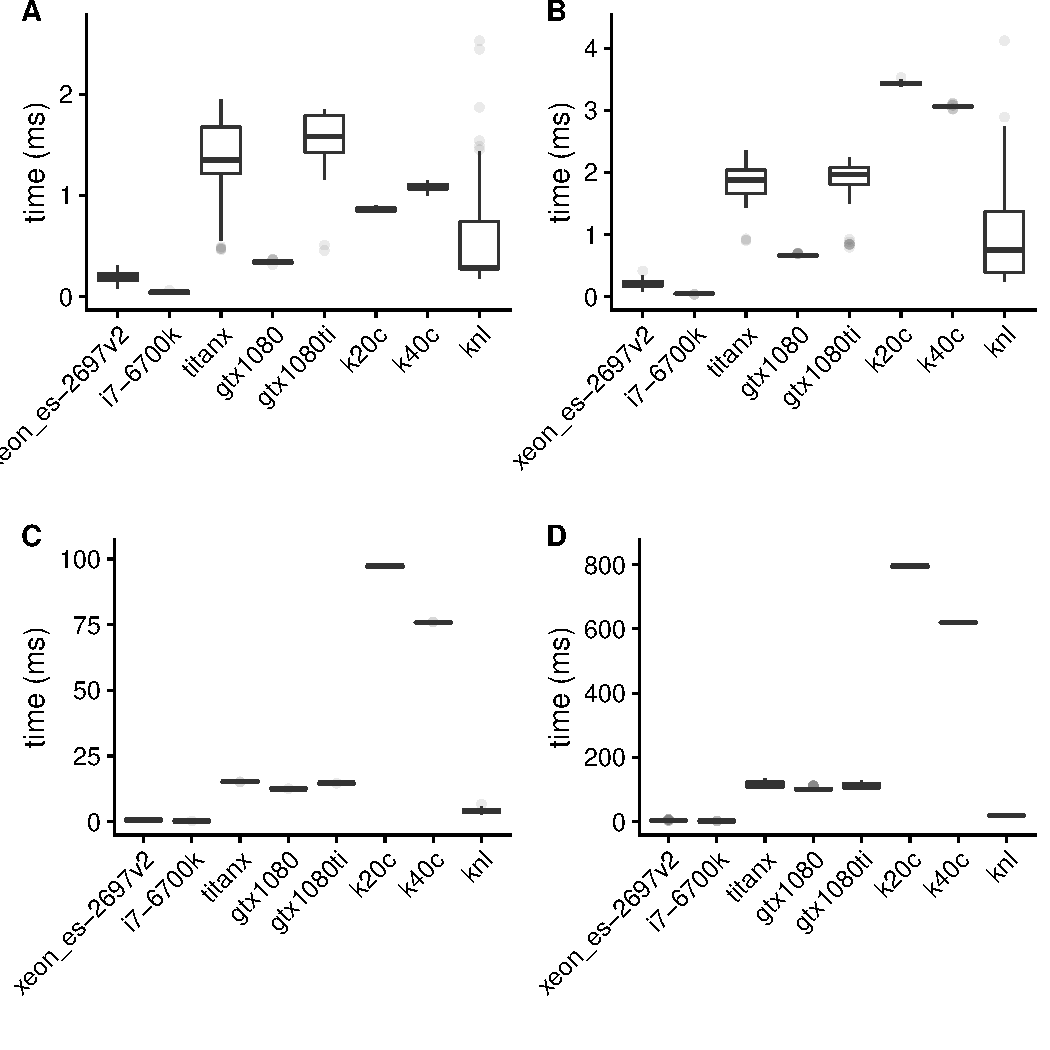
\includegraphics[width=\textwidth]{figures/time-results/crc.pdf}
\caption{Kernel Execution times for {\bf crc}, the only application favouring the CPU architectures.}
\label{fig:time-crc}
\end{minipage}
\end{figure}
Where $\Phi$ is substituted as the argument for each benchmark, it is taken as the respective scale from Table~\ref{tab:problem_sizes} and is inserted into Table~\ref{tab:program_arguments}.

Each {\bf Device} can be selected in a uniform way between applications using the same notation, on this system {\bf Device} comprises of {\tt -p 1 -d 0 -t 0} for the Intel Skylake CPU, where {\tt p} and {\tt d} are the integer identifier of the platform and device to respectively use, and {\tt -p 1 -d 0 -t 1} for the Nvidia Geforce GTX 1080 GPU.
Each application is run as {\bf Benchmark} {\bf Device} {\tt --} {\bf Arguments}, where {\bf Arguments} is taken from Table~\ref{tab:program_arguments} at the selected scale of $\Phi$.
For reproducibility the entire set of python scripts with all problem sizes is available in a Github repository~\cite{johnston2017}. 

\end{document}
